\documentclass[tikz,border=2pt]{standalone}
\usetikzlibrary{arrows.meta,positioning,calc,shapes.geometric}
\usepackage{fontspec}
\setmainfont{TeX Gyre Termes}
\setsansfont{Roboto}
\begin{document}
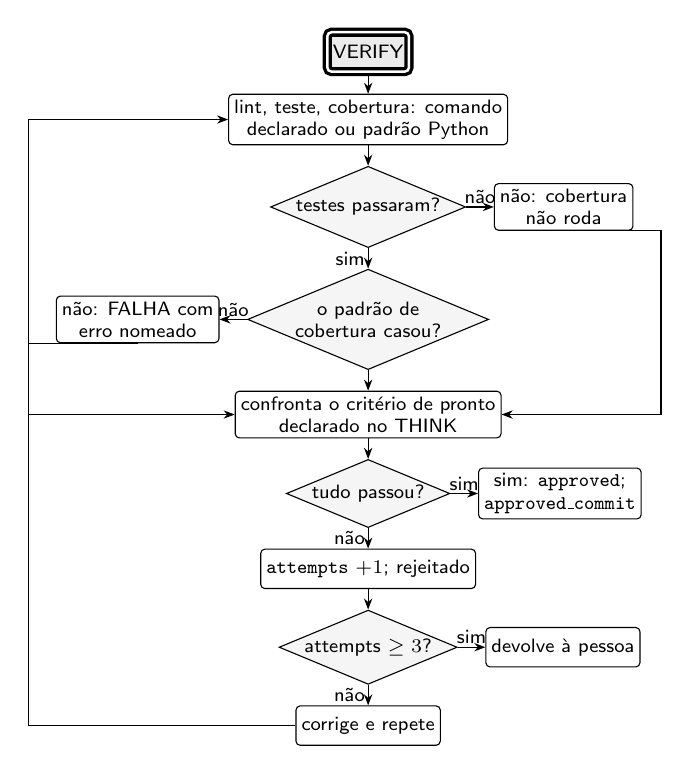
\begin{tikzpicture}[
  font=\sffamily\scriptsize, >={Stealth[length=4pt]},
  proc/.style={draw, thin, rounded corners=1.5pt, align=center, fill=white, minimum height=0.5cm, inner sep=2pt},
  exec/.style={proc, very thick, double distance=0.9pt, fill=black!8},
  dec/.style={draw, thin, diamond, aspect=2.4, align=center, fill=black!4, inner sep=0.5pt, font=\sffamily\scriptsize},
  nota/.style={font=\sffamily\scriptsize, align=center, text=black!80},
  lbl/.style={font=\sffamily\scriptsize, inner sep=1pt}
]
\node[exec] (a) {VERIFY};
\node[proc, below=0.26cm of a] (run) {lint, teste, cobertura: comando\\ declarado ou padrão Python};
\node[dec, below=0.26cm of run] (tp) {testes passaram?};
\node[proc, right=0.35cm of tp] (skip) {não: cobertura\\ não roda};
\node[dec, below=0.26cm of tp] (cp) {o padrão de\\ cobertura casou?};
\node[proc, left=0.35cm of cp] (fail) {não: FALHA com\\ erro nomeado};
\node[proc, below=0.26cm of cp] (crit) {confronta o critério de pronto\\ declarado no THINK};
\node[dec, below=0.26cm of crit] (ok) {tudo passou?};
\node[proc, right=0.35cm of ok] (ap) {sim: \texttt{approved};\\ \texttt{approved\_commit}};
\node[proc, below=0.26cm of ok] (rej) {\texttt{attempts} $+1$; rejeitado};
\node[dec, below=0.26cm of rej] (hb) {attempts $\ge 3$?};
\node[proc, right=0.35cm of hb] (hand) {devolve à pessoa};
\node[proc, below=0.26cm of hb] (fix) {corrige e repete};
% canais laterais: L desce a esquerda de tudo, R a direita de tudo,
% para que nenhuma linha de retorno atravesse as caixas centrais.
\coordinate (L) at ($(fail.west)+(-0.35,0)$);
\coordinate (R) at ($(skip.east)+(0.35,0)$);
\draw[->] (a) -- (run);
\draw[->] (run) -- (tp);
\draw[->] (tp) -- node[lbl,above]{não} (skip);
\draw[->] (tp) -- node[lbl,left]{sim} (cp);
\draw[->] (cp) -- node[lbl,above]{não} (fail);
\draw[->] (cp) -- (crit);
\draw[->] (skip.south) -- (skip.south -| R) -- (crit.east -| R) -- (crit.east);
\draw[->] (fail.south) -- (fail.south -| L) -- (crit.west -| L) -- (crit.west);
\draw[->] (crit) -- (ok);
\draw[->] (ok) -- node[lbl,above]{sim} (ap);
\draw[->] (ok) -- node[lbl,left]{não} (rej);
\draw[->] (rej) -- (hb);
\draw[->] (hb) -- node[lbl,above]{sim} (hand);
\draw[->] (hb) -- node[lbl,left]{não} (fix);
\draw[->] (fix.west) -- (fix.west -| L) -- (run.west -| L) -- (run.west);
\end{tikzpicture}
\end{document}
